\documentclass[aspectratio=169, 10pt]{beamer}

% -----------------------------------------------------------------------------
% Theme & Styling
% -----------------------------------------------------------------------------
\usetheme{Madrid}
\usecolortheme{whale}

% Custom Colors (Academic Navy & Modern Accents)
\definecolor{usthblue}{RGB}{11, 60, 93}
\definecolor{usthaccent}{RGB}{42, 120, 214}
\definecolor{darkslate}{RGB}{30, 41, 59}
\definecolor{accentorange}{RGB}{235, 104, 52}
\definecolor{accentgreen}{RGB}{27, 175, 122}
\definecolor{lightgrey}{RGB}{245, 247, 250}

\setbeamercolor{palette primary}{bg=usthblue,fg=white}
\setbeamercolor{palette secondary}{bg=usthaccent,fg=white}
\setbeamercolor{palette tertiary}{bg=darkslate,fg=white}
\setbeamercolor{structure}{fg=usthblue}
\setbeamercolor{titlelike}{parent=palette primary}
\setbeamercolor{block title}{bg=usthblue,fg=white}
\setbeamercolor{block body}{bg=lightgrey,fg=darkslate}
\setbeamercolor{block title example}{bg=accentgreen,fg=white}
\setbeamercolor{block body example}{bg=lightgrey,fg=darkslate}
\setbeamercolor{block title alerted}{bg=accentorange,fg=white}
\setbeamercolor{block body alerted}{bg=lightgrey,fg=darkslate}

\setbeamertemplate{navigation symbols}{}
\setbeamertemplate{itemize items}[circle]

% -----------------------------------------------------------------------------
% Packages
% -----------------------------------------------------------------------------
\usepackage[utf8]{inputenc}
\usepackage{graphicx}
\usepackage{booktabs}
\usepackage{amsmath,amssymb}
\usepackage{multicol}
\usepackage{colortbl}
\usepackage{tikz}

% -----------------------------------------------------------------------------
% Metadata
% -----------------------------------------------------------------------------
\title[Compression in Spark over HDFS]{Experimental Evaluation of Data Compression\\in Spark over HDFS}
\subtitle{Storage vs. Communication Trade-offs on a Heterogeneous Cluster}
\author[USTH InfraCloud]{InfraCloud Project Team}
\institute[USTH]{
  Master 2 -- Cloud Computing \& Big Data\\
  University of Science and Technology of Hanoi (USTH)
}
\date{\today}

% -----------------------------------------------------------------------------
% Document
% -----------------------------------------------------------------------------
\begin{document}

% -----------------------------------------------------------------------------
% Slide 1: Title
% -----------------------------------------------------------------------------
\begin{frame}[plain]
  \titlepage
\end{frame}

% -----------------------------------------------------------------------------
% Slide 2: Context, Motivation & Problem Statement
% -----------------------------------------------------------------------------
\begin{frame}{Context, Motivation \& Problem Statement}
  \begin{columns}[T]
    \begin{column}{0.55\textwidth}
      \begin{block}{The Fundamental Trade-off}
        \textbf{Compression is not a free lunch:}
        \begin{itemize}
          \item Trades \textbf{CPU cycles} for \textbf{fewer bytes} on disk and wire.
          \item Big Data pipelines balance CPU capacity, disk I/O throughput, and network bandwidth.
        \end{itemize}
      \end{block}

      \begin{block}{Two Compression Tiers in Spark}
        \begin{itemize}
          \item \textbf{Storage-level:} Persistent Parquet data at rest in HDFS (input reads \& job writes).
          \item \textbf{Communication-level:} Intermediate shuffle blocks, spill files, and broadcast variables across executors.
        \end{itemize}
      \end{block}
    \end{column}

    \begin{column}{0.43\textwidth}
      \begin{alertblock}{Core Research Question}
        Under what \textbf{hardware bottlenecks}, \textbf{workload profiles}, and \textbf{dataset sizes} does compression accelerate execution, and under what conditions does it become counterproductive?
      \end{alertblock}

      \vspace{0.2cm}
      \centering
      \small
      \textbf{Key Approach:}\\
      Rigorous experimental evaluation across 300 runs on a 2-node heterogeneous cluster using real NYC Taxi data.
    \end{column}
  \end{columns}
\end{frame}

% -----------------------------------------------------------------------------
% Slide 3: Experimental Infrastructure & Reproducibility
% -----------------------------------------------------------------------------
\begin{frame}{Experimental Infrastructure \& Reproducibility}
  \begin{columns}[T]
    \begin{column}{0.55\textwidth}
      \textbf{Heterogeneous 2-Node Cluster (20 Cores):}
      \begin{itemize}
        \item \textbf{PC (Ubuntu Linux x86, i5-13500, 20 threads, 62 GB):}
          \begin{itemize}
            \footnotesize
            \item NameNode, DataNode, Spark Master, Prometheus, Grafana.
            \item \textbf{4 identical workers} (4 cores / 5 GB heap each) = 16 cores.
          \end{itemize}
        \item \textbf{MacBook Pro (Apple Silicon M1 Pro, 16 GB):}
          \begin{itemize}
            \footnotesize
            \item DataNode, \textbf{1 worker} (4 cores / 5 GB heap) in Docker VM.
          \end{itemize}
        \item \textbf{Network Interconnect:} Real-world home Wi-Fi LAN.
          \begin{itemize}
            \footnotesize
            \item Mac $\rightarrow$ PC: \textbf{310--350 Mbit/s} | PC $\rightarrow$ Mac: \textbf{550--670 Mbit/s}.
            \item Asymmetric, bandwidth-constrained (primary cluster bottleneck).
          \end{itemize}
      \end{itemize}
    \end{column}

    \begin{column}{0.43\textwidth}
      \begin{block}{Scientific Reproducibility}
        \begin{itemize}
          \footnotesize
          \item \textbf{Frozen Baseline:} Pinned \texttt{spark-defaults.conf}. Dynamic allocation, AQE, broadcast joins, and speculation disabled.
          \item \textbf{No Cache Pollution:} Linux OS page caches dropped on \textit{both} hosts before every run.
          \item \textbf{Observability:} Prometheus scrapes node-exporter (CPU, disk, net) and cAdvisor every 2 s + Spark EventLog metrics.
        \end{itemize}
      \end{block}
    \end{column}
  \end{columns}
\end{frame}

% -----------------------------------------------------------------------------
% Slide 4: Workload Design & Characterization Gate
% -----------------------------------------------------------------------------
\begin{frame}{Workload Design \& Characterization Gate}
  \small
  All workloads read the same NYC TLC Yellow Taxi dataset (525.6M rows, 18 columns).
  \vspace{0.15cm}

  \begin{table}
    \centering
    \footnotesize
    \begin{tabular}{llcccc}
      \toprule
      \textbf{App} & \textbf{Algorithm / Operation} & \textbf{CPU Util.} & \textbf{Link Airtime} & \textbf{Shuffle} & \textbf{Profile} \\
      \midrule
      \textbf{A1} & \texttt{IoBoundEtl}: Repartition by date & 6--7\% & \textbf{102--107\%} & 22.5--44.9 GB & \textbf{I/O-bound} \\
      \textbf{A2} & \texttt{CpuBoundKMeans}: $k=1024$, 8 features & \textbf{65--80\%} & 13--19\% & 0 GB & \textbf{CPU-bound} \\
      \textbf{A3} & \texttt{BalancedRouteStats}: Aggregates + sort & 41--46\% & 47--61\% & 2.1--4.1 GB & \textbf{Balanced} \\
      \bottomrule
    \end{tabular}
  \end{table}

  \begin{columns}[onlytextwidth]
    \begin{column}{0.31\textwidth}
      \begin{block}{\footnotesize A1: I/O-Bound}
        \scriptsize
        Executors idle $>90\%$ of time waiting on saturated Wi-Fi link. Shuffle volume is $4.3\times$ input size.
      \end{block}
    \end{column}
    \hfill
    \begin{column}{0.31\textwidth}
      \begin{block}{\footnotesize A2: CPU-Bound}
        \scriptsize
        $13/16$ PC cores busy. No shuffle, negligible network ($<1$ GB). Compute per row dwarfs input read.
      \end{block}
    \end{column}
    \hfill
    \begin{column}{0.31\textwidth}
      \begin{block}{\footnotesize A3: Balanced}
        \scriptsize
        Multi-moment aggregates over route $\times$ 6h day-part. Moderate CPU and network; neither saturated.
      \end{block}
    \end{column}
  \end{columns}
\end{frame}

% -----------------------------------------------------------------------------
% Slide 5: Intrinsic Codec Characteristics (Experiment E0)
% -----------------------------------------------------------------------------
\begin{frame}{Intrinsic Codec Characteristics (Experiment E0)}
  \begin{columns}[T]
    \begin{column}{0.5\textwidth}
      \textbf{Standalone JVM Microbenchmark (E0):}
      \begin{itemize}
        \footnotesize
        \item Single-threaded in-memory benchmark on PC \& Mac.
        \item Tests 134 MB Parquet sample vs 256 MB CSV text.
      \end{itemize}

      \vspace{0.1cm}
      \begin{block}{\footnotesize Key E0 Findings}
        \begin{itemize}
          \scriptsize
          \item \textbf{Three Tiers:}
            \begin{itemize}
              \scriptsize
              \item \textit{Lightweight:} Snappy \& LZ4 ($\sim$800 MB/s, ratio 1.43$\times$).
              \item \textit{Dominant:} \textbf{Zstd} (1.85--2.26$\times$, 274 MB/s at level 3).
              \item \textit{Heavyweight:} Gzip (1.81$\times$, slow 7--80 MB/s).
            \end{itemize}
          \item \textbf{Zstd dominates Gzip outright:} Zstd-3 is \textbf{10$\times$ faster compressing} and \textbf{4$\times$ faster decompressing} than Gzip-6, with higher ratio.
          \item \textbf{Data Format Impact:} Uncompressed Parquet achieves 1.4--2.3$\times$ (already dictionary/RLE encoded); raw CSV achieves 2.5--5.7$\times$.
        \end{itemize}
      \end{block}
    \end{column}

    \begin{column}{0.48\textwidth}
      \centering
      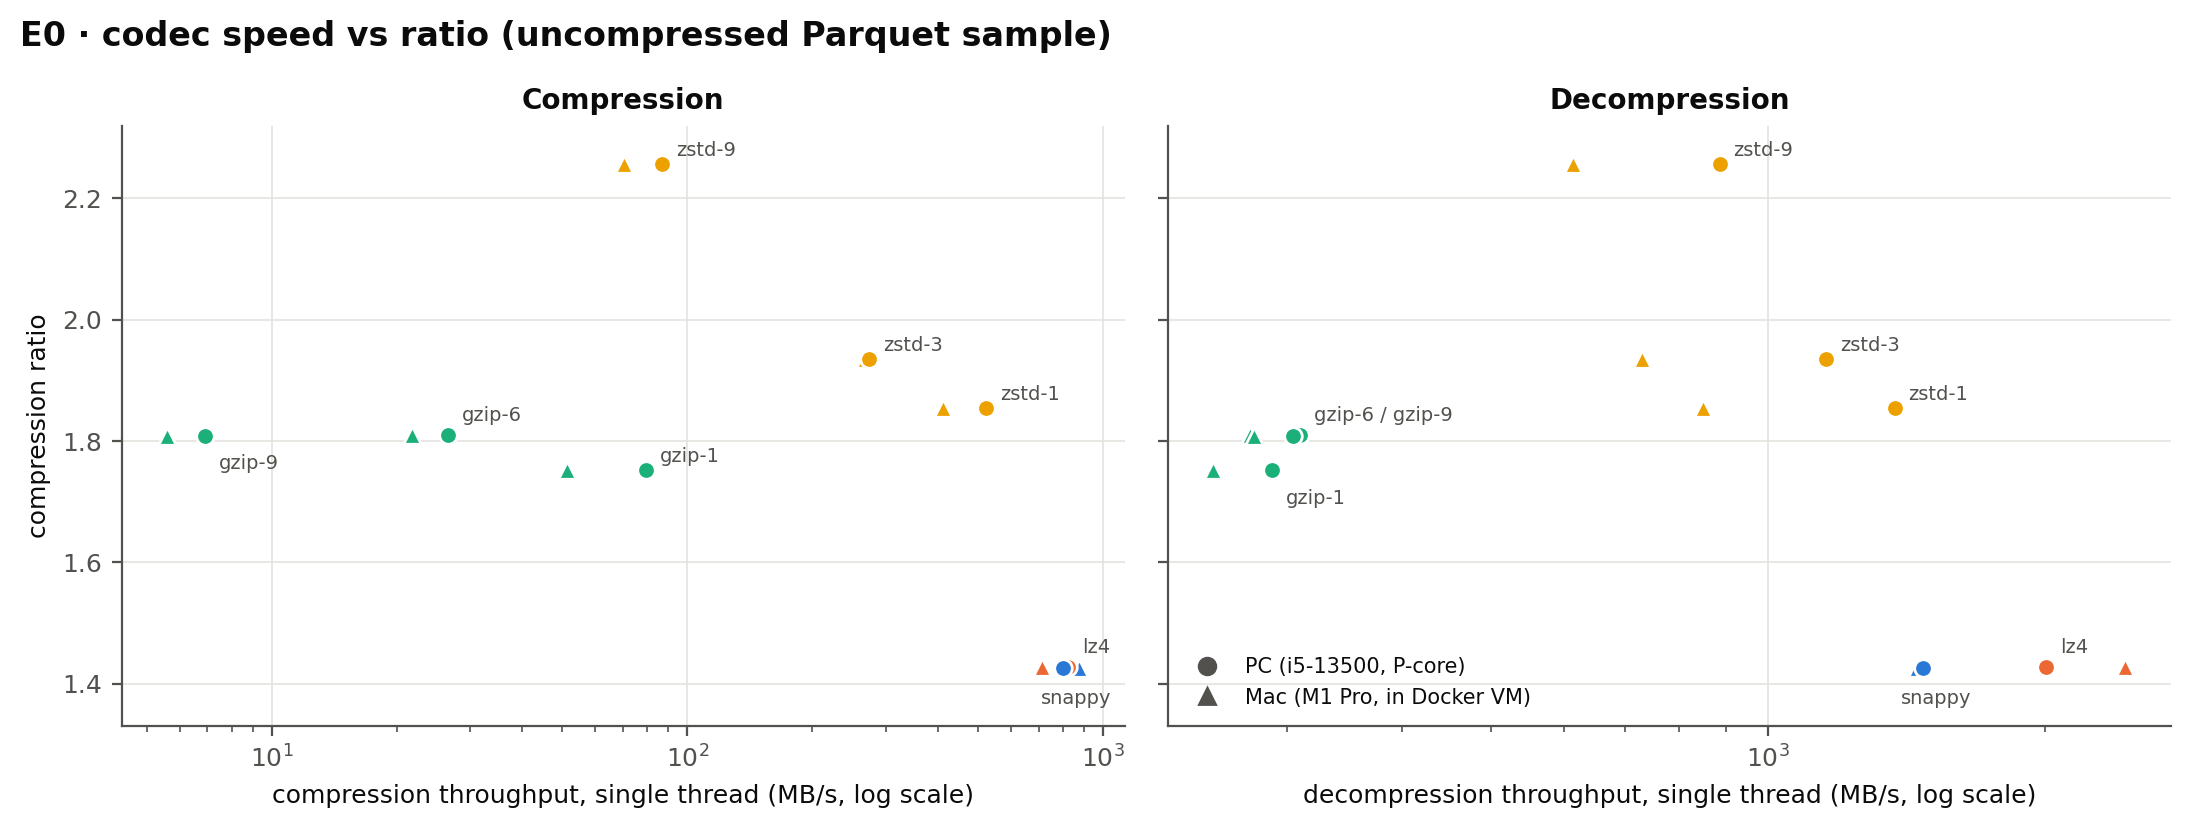
\includegraphics[width=\textwidth,height=0.72\textheight,keepaspectratio]{../results/plots/fig8_e0_speed_vs_ratio.png}
    \end{column}
  \end{columns}
\end{frame}

% -----------------------------------------------------------------------------
% Slide 6: The Compression Matrix (C0 to C3) & Campaign
% -----------------------------------------------------------------------------
\begin{frame}{The Compression Matrix (C0 to C3) \& Campaign Design}
  % Table spanning the full slide width to avoid any column overlap
  \begin{table}
    \centering
    \footnotesize
    \begin{tabular}{lllc}
      \toprule
      \textbf{Configuration} & \textbf{Storage Level (Parquet)} & \textbf{Shuffle Level (Comm.)} & \textbf{Variants} \\
      \midrule
      \textbf{C0 (Baseline)} & Uncompressed & Disabled & 1 \\
      \textbf{C1 (Storage-only)} & Snappy, LZ4, Gzip, Zstd & Disabled & 4 \\
      \textbf{C2 (Shuffle-only)} & Uncompressed & LZ4, Snappy, Zstd & 3 \\
      \textbf{C3 (Combined)} & Snappy+LZ4 (fast) / Gzip+Zstd (heavy) & Enabled (both levels) & 2 \\
      \bottomrule
    \end{tabular}
  \end{table}

  \vspace{0.15cm}

  \begin{columns}[T]
    \begin{column}{0.48\textwidth}
      \begin{block}{Rigorous Experimental Campaign}
        \begin{itemize}
          \footnotesize
          \item \textbf{Matrix Scope:} 4 sizes (0.5, 2.5, 5, 10 GB) $\times$ 25 app-configs $\times$ 3 reps = \textbf{300 runs}.
          \item \textbf{High Reliability:} 100\% successful runs (0 failures).
          \item \textbf{Repeatability:} Median CV = \textbf{2.5\%}.
        \end{itemize}
      \end{block}
    \end{column}

    \begin{column}{0.48\textwidth}
      \begin{alertblock}{Significance Decision Rule}
        \footnotesize
        Two configurations are called \textbf{significantly different} only when their \textbf{min..max ranges over 3 runs do not overlap}. Otherwise reported as a \textit{trend}.
      \end{alertblock}

      \vspace{0.1cm}
      \begin{block}{\footnotesize Scope Note}
        \scriptsize
        Spark does not support Gzip for shuffle compression (C2 has 3 variants). A2 has no shuffle, so only C0 and C1 are run.
      \end{block}
    \end{column}
  \end{columns}
\end{frame}

% -----------------------------------------------------------------------------
% Slide 7: Storage-Level Compression (C1) Results
% -----------------------------------------------------------------------------
\begin{frame}{Storage-Level Compression (C1) Results}
  \begin{columns}[T]
    \begin{column}{0.48\textwidth}
      \centering
      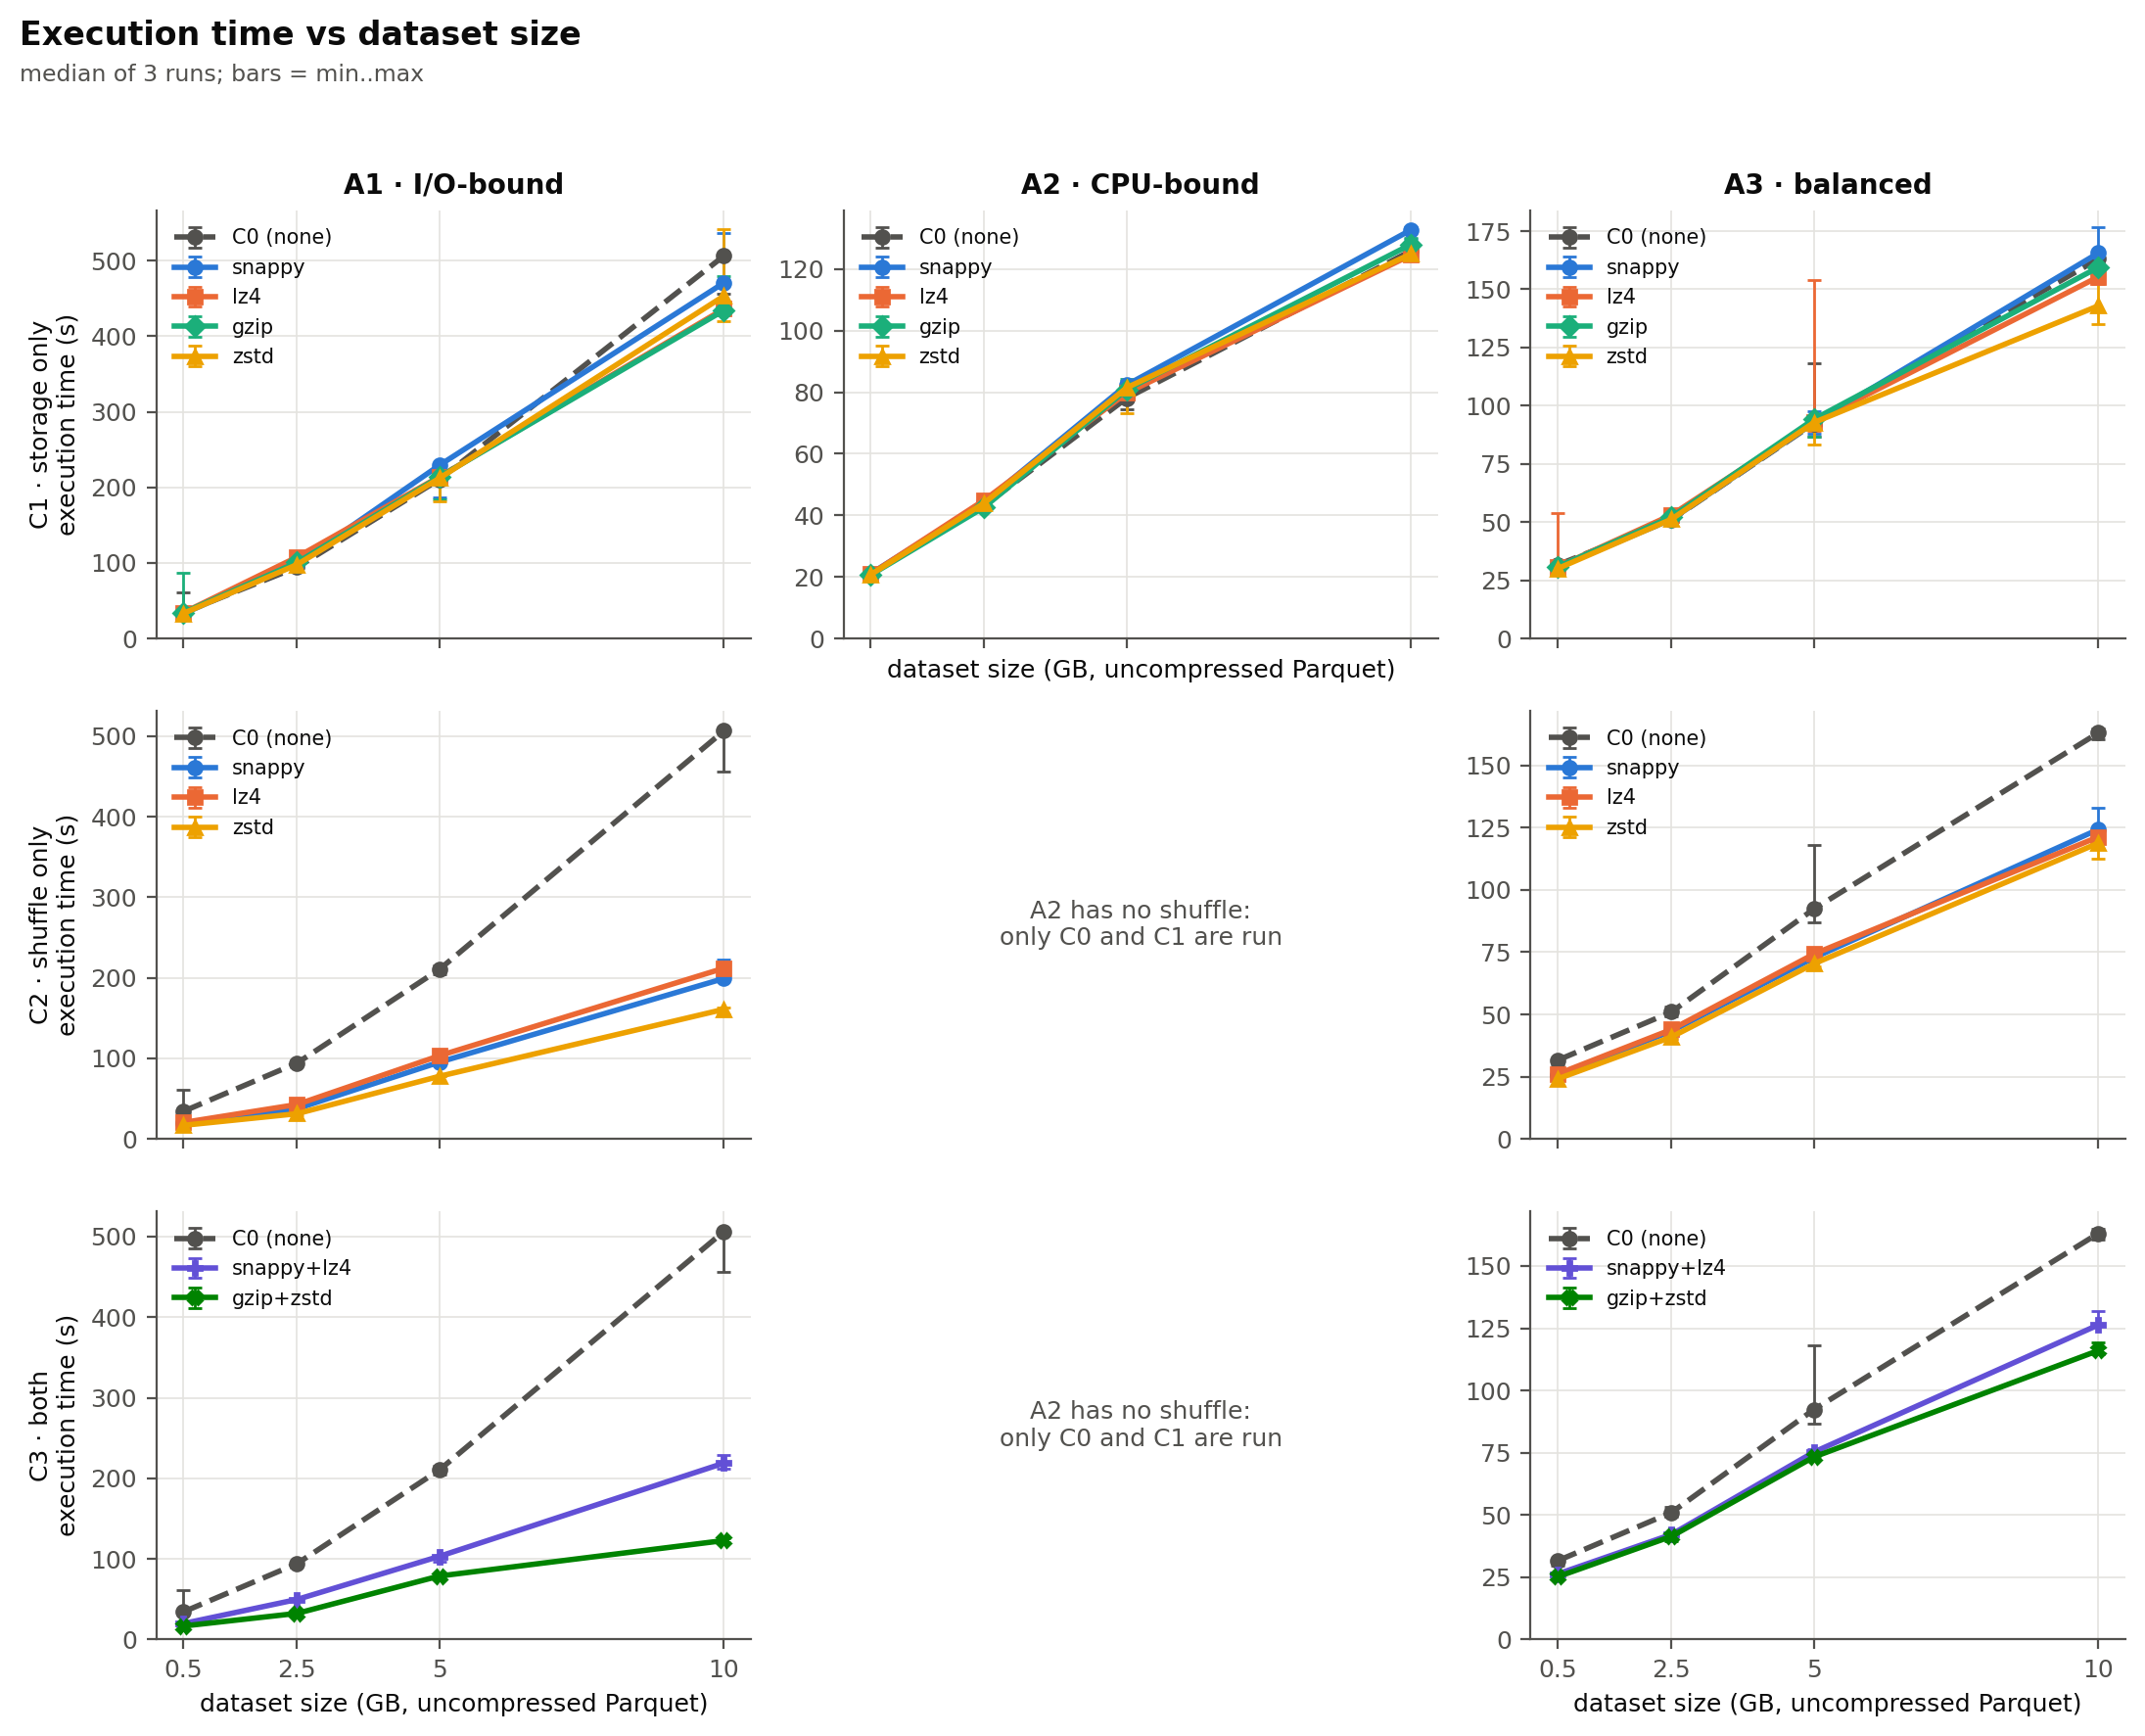
\includegraphics[width=\textwidth]{../results/plots/fig1_time_vs_size.png}
    \end{column}

    \begin{column}{0.5\textwidth}
      \textbf{Impact of Compressing HDFS Data at Rest:}
      \begin{itemize}
        \footnotesize
        \item \textbf{Disk Space Savings:} Shrinks Parquet footprint by 30\% (Snappy/LZ4) to 47\% (Zstd).
        \item \textbf{Does disk I/O savings compensate for CPU overhead?}
          \begin{itemize}
            \scriptsize
            \item \textbf{Below 10 GB: No.} Codecs were 4--12\% \textit{slower} on A1 at 2.5 GB. 91\% of tasks read local NVMe blocks---input I/O is not on the critical path.
            \item \textbf{At 10 GB: Trend emerges.} A1 end-to-end shows a 1.08--1.17$\times$ speed-up (trend; overlaps C0 spread). Map-stage read is significantly faster (49--59 s vs 85 s). A3 gains a significant 1.14$\times$ with Zstd.
          \end{itemize}
        \item \textbf{Gzip Inefficiency:} Gzip adds \textbf{+62\% executor CPU} on A1 at 10 GB with zero runtime advantage over Zstd.
      \end{itemize}
    \end{column}
  \end{columns}
\end{frame}

% -----------------------------------------------------------------------------
% Slide 8: Communication-Level Compression (C2) Results
% -----------------------------------------------------------------------------
\begin{frame}{Communication-Level Compression (C2) Results}
  \begin{columns}[T]
    \begin{column}{0.48\textwidth}
      \centering
      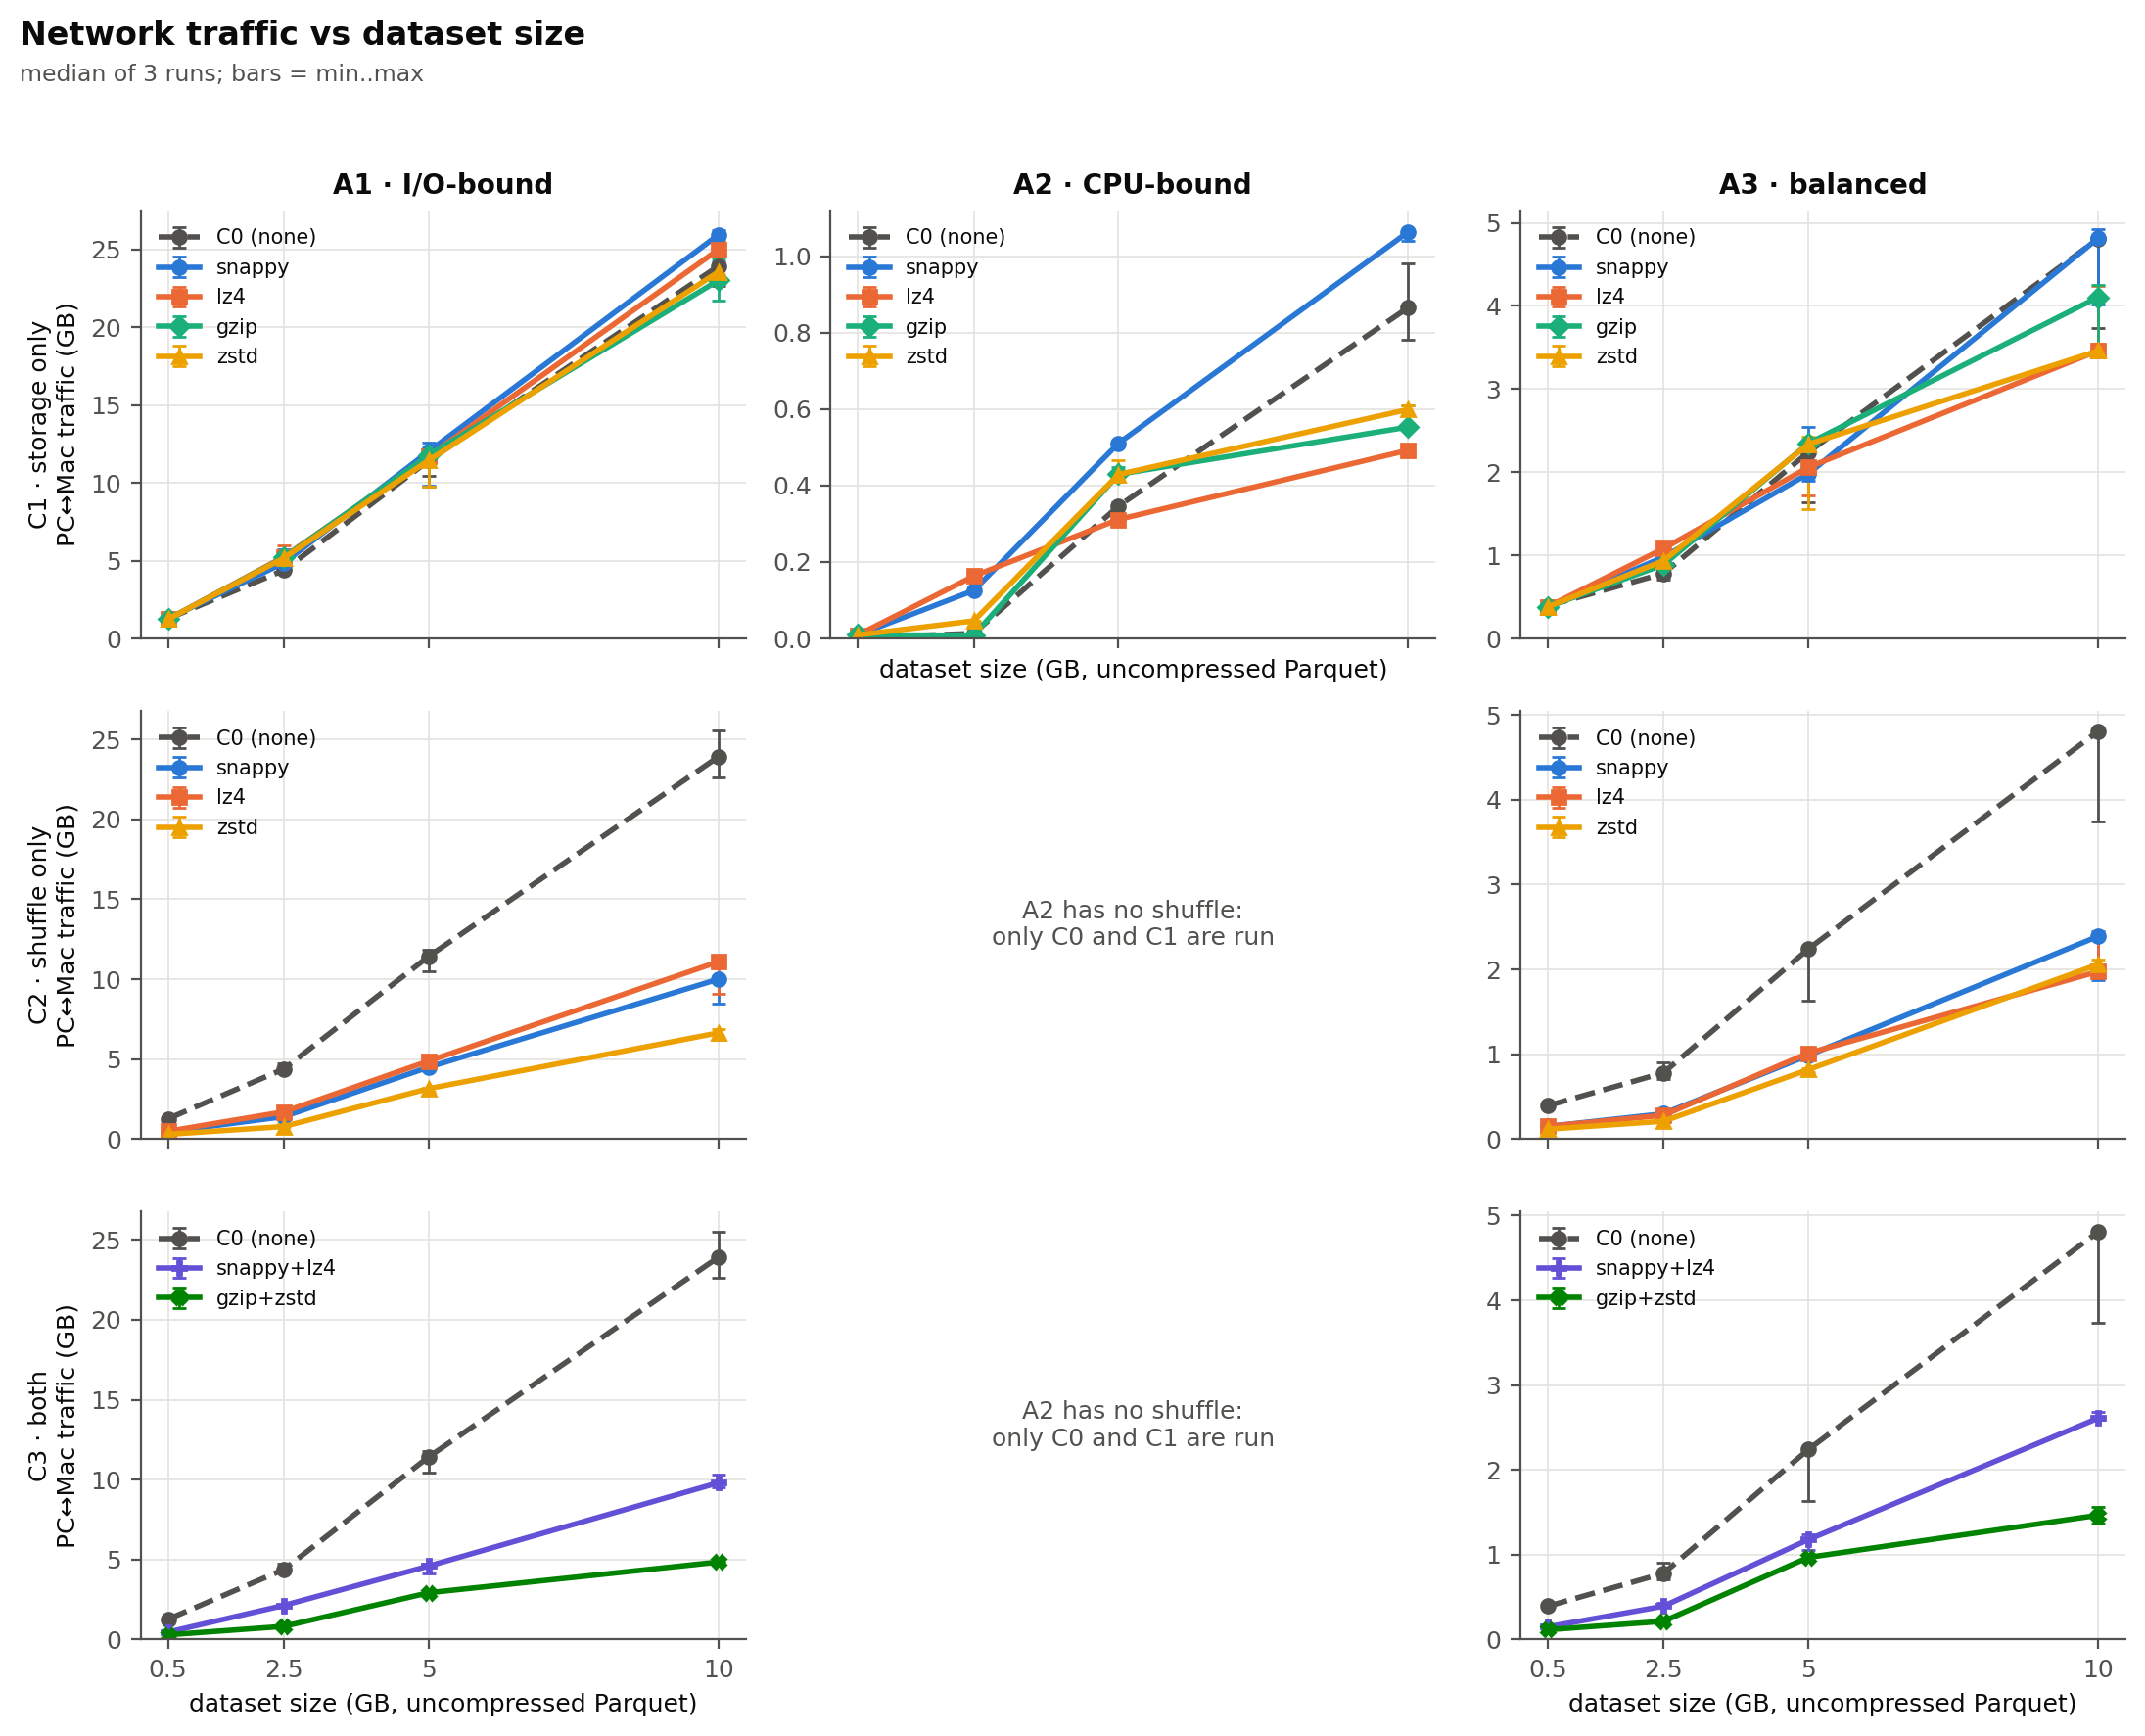
\includegraphics[width=\textwidth]{../results/plots/fig4_network_vs_size.png}
    \end{column}

    \begin{column}{0.5\textwidth}
      \textbf{Massive Speed-up from Shuffle Compression:}
      \begin{itemize}
        \footnotesize
        \item \textbf{High Compressibility:} Row-format shuffle blocks compress \textbf{2.8--4.8$\times$} (A1) and \textbf{2.7--3.5$\times$} (A3).
        \item \textbf{Dramatic Wall-Clock Reduction (A1 @ 10 GB):}
          \begin{itemize}
            \scriptsize
            \item C0: 506 s $\rightarrow$ LZ4: 212 s (\textbf{2.39$\times$})
            \item Snappy: 199 s (\textbf{2.54$\times$}) $\rightarrow$ Zstd: 161 s (\textbf{3.15$\times$})
          \end{itemize}
        \item \textbf{Fetch-Wait Collapse:} Reducer fetch-wait time falls \textbf{9$\times$} (7,396 s $\rightarrow$ 848 s with Zstd).
        \item \textbf{Negligible CPU Overhead:} LZ4/Snappy add +4\% CPU; Zstd adds +26\% CPU, which is repaid many times over by removing 72\% of network traffic.
        \item \textbf{Verdict:} Shuffle compression was \textbf{never counterproductive}.
      \end{itemize}
    \end{column}
  \end{columns}
\end{frame}

% -----------------------------------------------------------------------------
% Slide 9: Combined Compression (C3) & Configuration Comparison
% -----------------------------------------------------------------------------
\begin{frame}{Combined Compression (C3) \& Configuration Comparison}
  \begin{columns}[T]
    \begin{column}{0.52\textwidth}
      \centering
      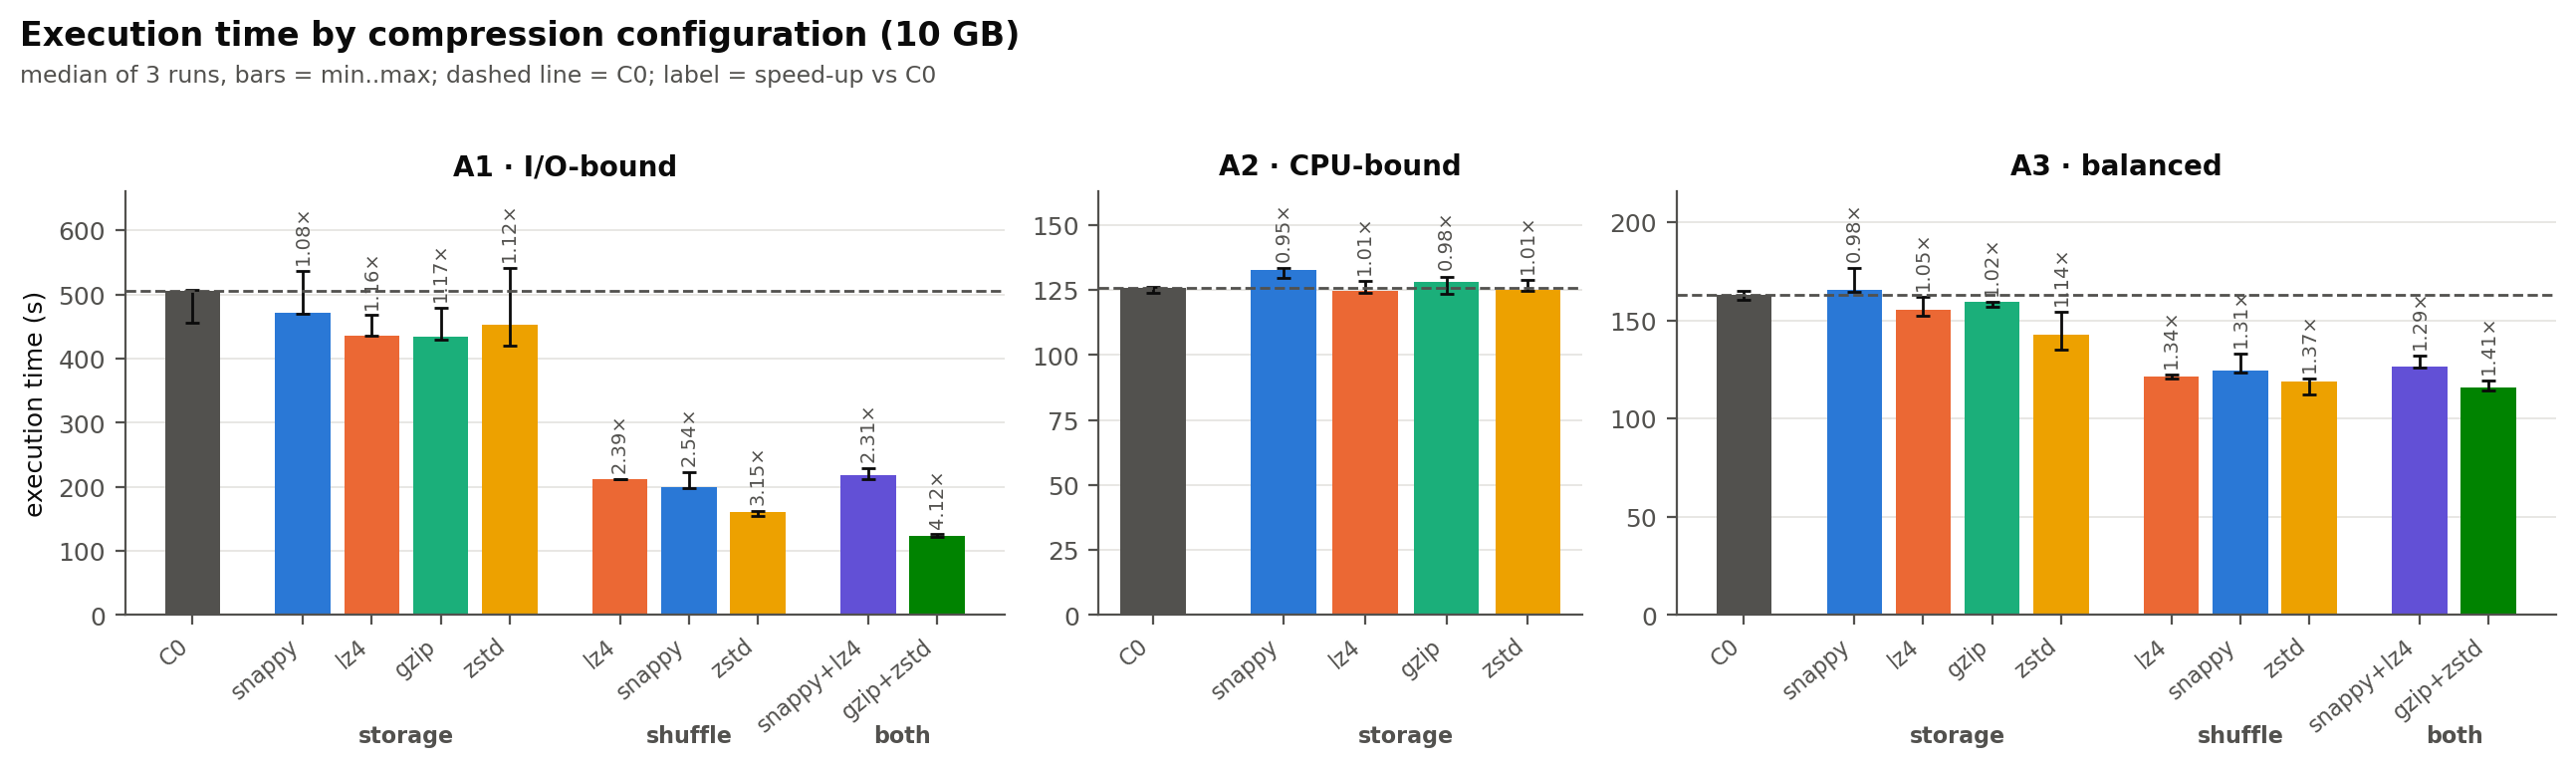
\includegraphics[width=\textwidth]{../results/plots/fig6_time_vs_config_10gb.png}
    \end{column}

    \begin{column}{0.46\textwidth}
      \textbf{When Do Both Levels Add Up?}
      \begin{itemize}
        \footnotesize
        \item \textbf{Below 10 GB: $C3 \approx C2$:}
          \begin{itemize}
            \scriptsize
            \item Within $\pm 4\%$ of shuffle-only. Adding storage compression adds CPU cost without reducing the bottleneck.
            \item Snappy+LZ4 is 16\% \textit{slower} at 2.5 GB.
          \end{itemize}
        \item \textbf{At 10 GB (The Inversion):}
          \begin{itemize}
            \scriptsize
            \item Heavy pair (\texttt{gzip+zstd}) achieves a \textbf{4.12$\times$ speed-up} on A1 (123 s vs 506 s C0 and 161 s C2-zstd).
            \item \textbf{Mechanism:} Storage compression relieves MacBook VM memory/disk pressure, while shuffle compression relieves the Wi-Fi link.
          \end{itemize}
        \item \textbf{Fast Pair Limitation:} \texttt{snappy+lz4} never beats LZ4 shuffle-only.
      \end{itemize}
    \end{column}
  \end{columns}
\end{frame}

% -----------------------------------------------------------------------------
% Slide 10: Impact of Dataset Size & Scaling
% -----------------------------------------------------------------------------
\begin{frame}{Impact of Dataset Size \& Scaling}
  \begin{columns}[T]
    \begin{column}{0.48\textwidth}
      \centering
      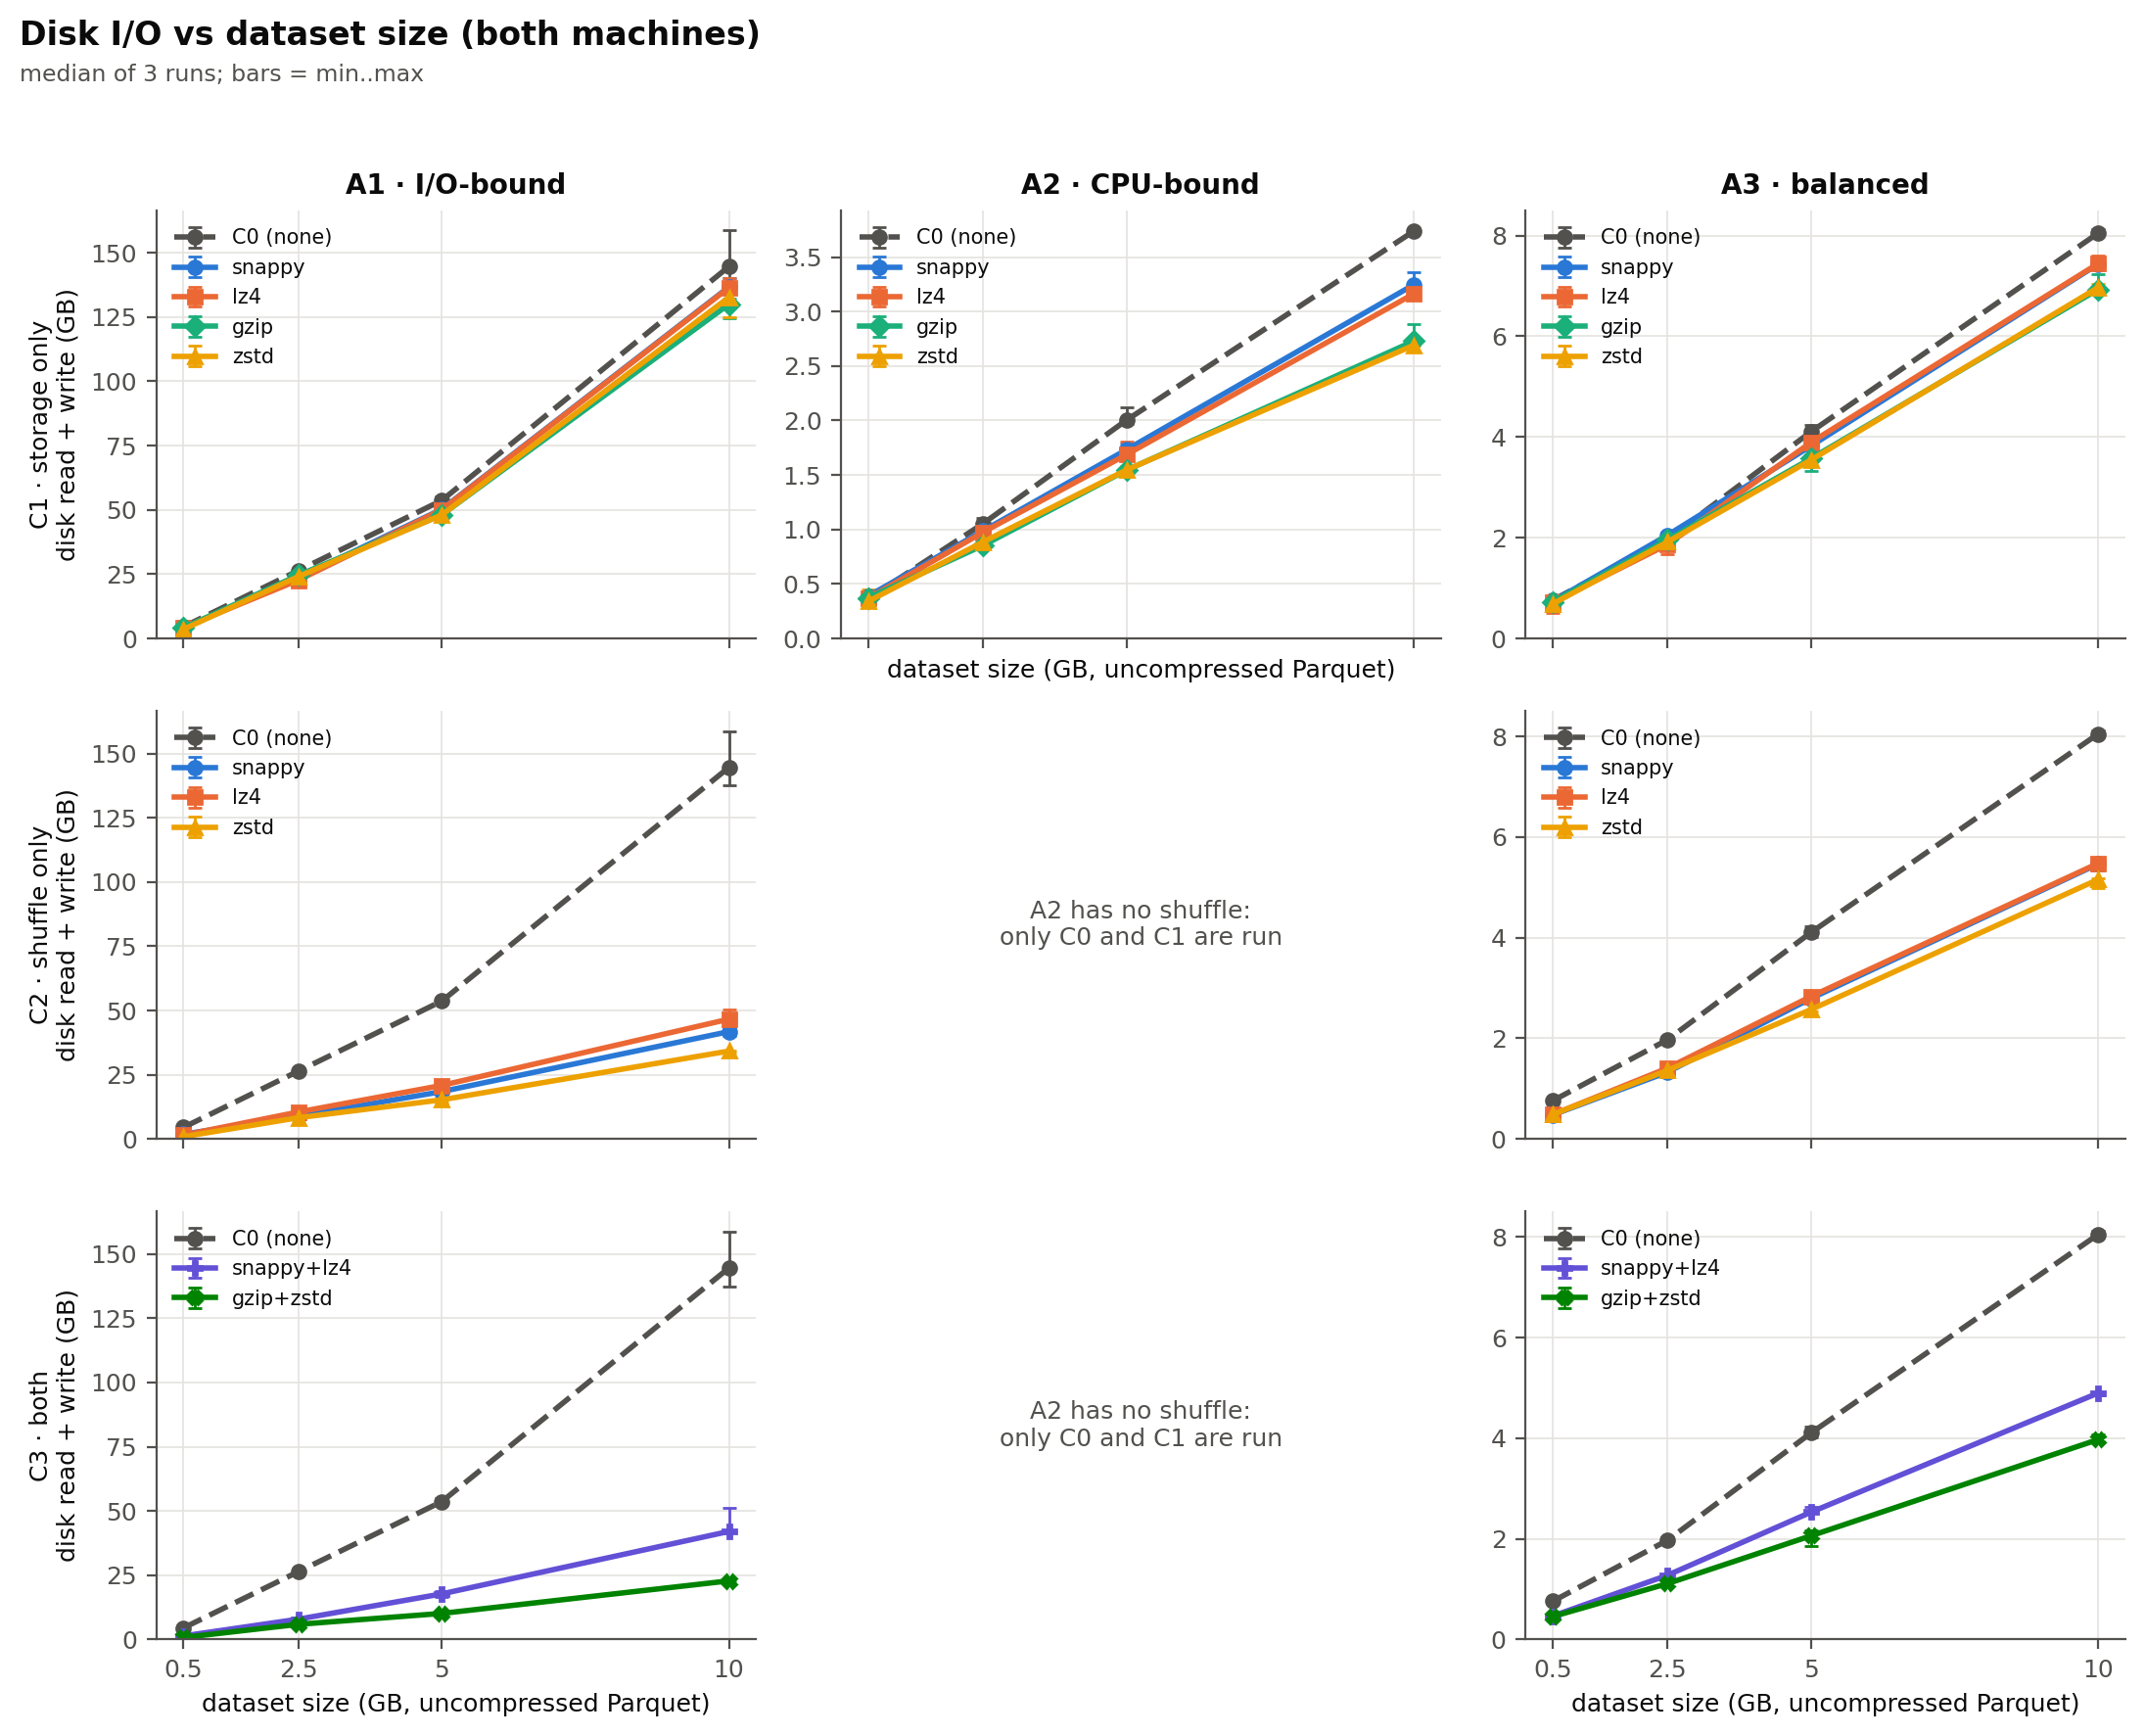
\includegraphics[width=\textwidth,height=0.74\textheight,keepaspectratio]{../results/plots/fig3_disk_vs_size.png}
    \end{column}

    \begin{column}{0.5\textwidth}
      \textbf{How Compression Benefits Evolve:}
      \begin{itemize}
        \footnotesize
        \item \textbf{Fixed Overhead Amortization:}
          \begin{itemize}
            \scriptsize
            \item At 0.5 GB, 10--15 s of fixed Spark startup and task scheduling dilutes relative speed-ups.
            \item At 10 GB, benefits scale cleanly with byte volume.
          \end{itemize}
        \item \textbf{The 10 GB VM Memory Threshold:}
          \begin{itemize}
            \scriptsize
            \item From 5 GB to 10 GB, input data doubles, but Mac disk reads spike \textbf{6$\times$} (4.6 $\rightarrow$ 28.1 GB).
            \item Mac VM's 10 GB RAM runs out of room for both working set and page cache; storage compression begins to matter.
          \end{itemize}
        \item \textbf{Algorithmic Ranking is Invariant:}
          \begin{itemize}
            \scriptsize
            \item Codec ratios and shuffle ranking ($Zstd > Snappy > LZ4$) remain perfectly stable across all dataset sizes.
          \end{itemize}
      \end{itemize}
    \end{column}
  \end{columns}
\end{frame}

% -----------------------------------------------------------------------------
% Slide 11: Workload Comparison & Answers to Q1--Q3
% -----------------------------------------------------------------------------
\begin{frame}{Workload Comparison \& Answers to Q1--Q3}
  \begin{columns}[T]
    \begin{column}{0.48\textwidth}
      \centering
      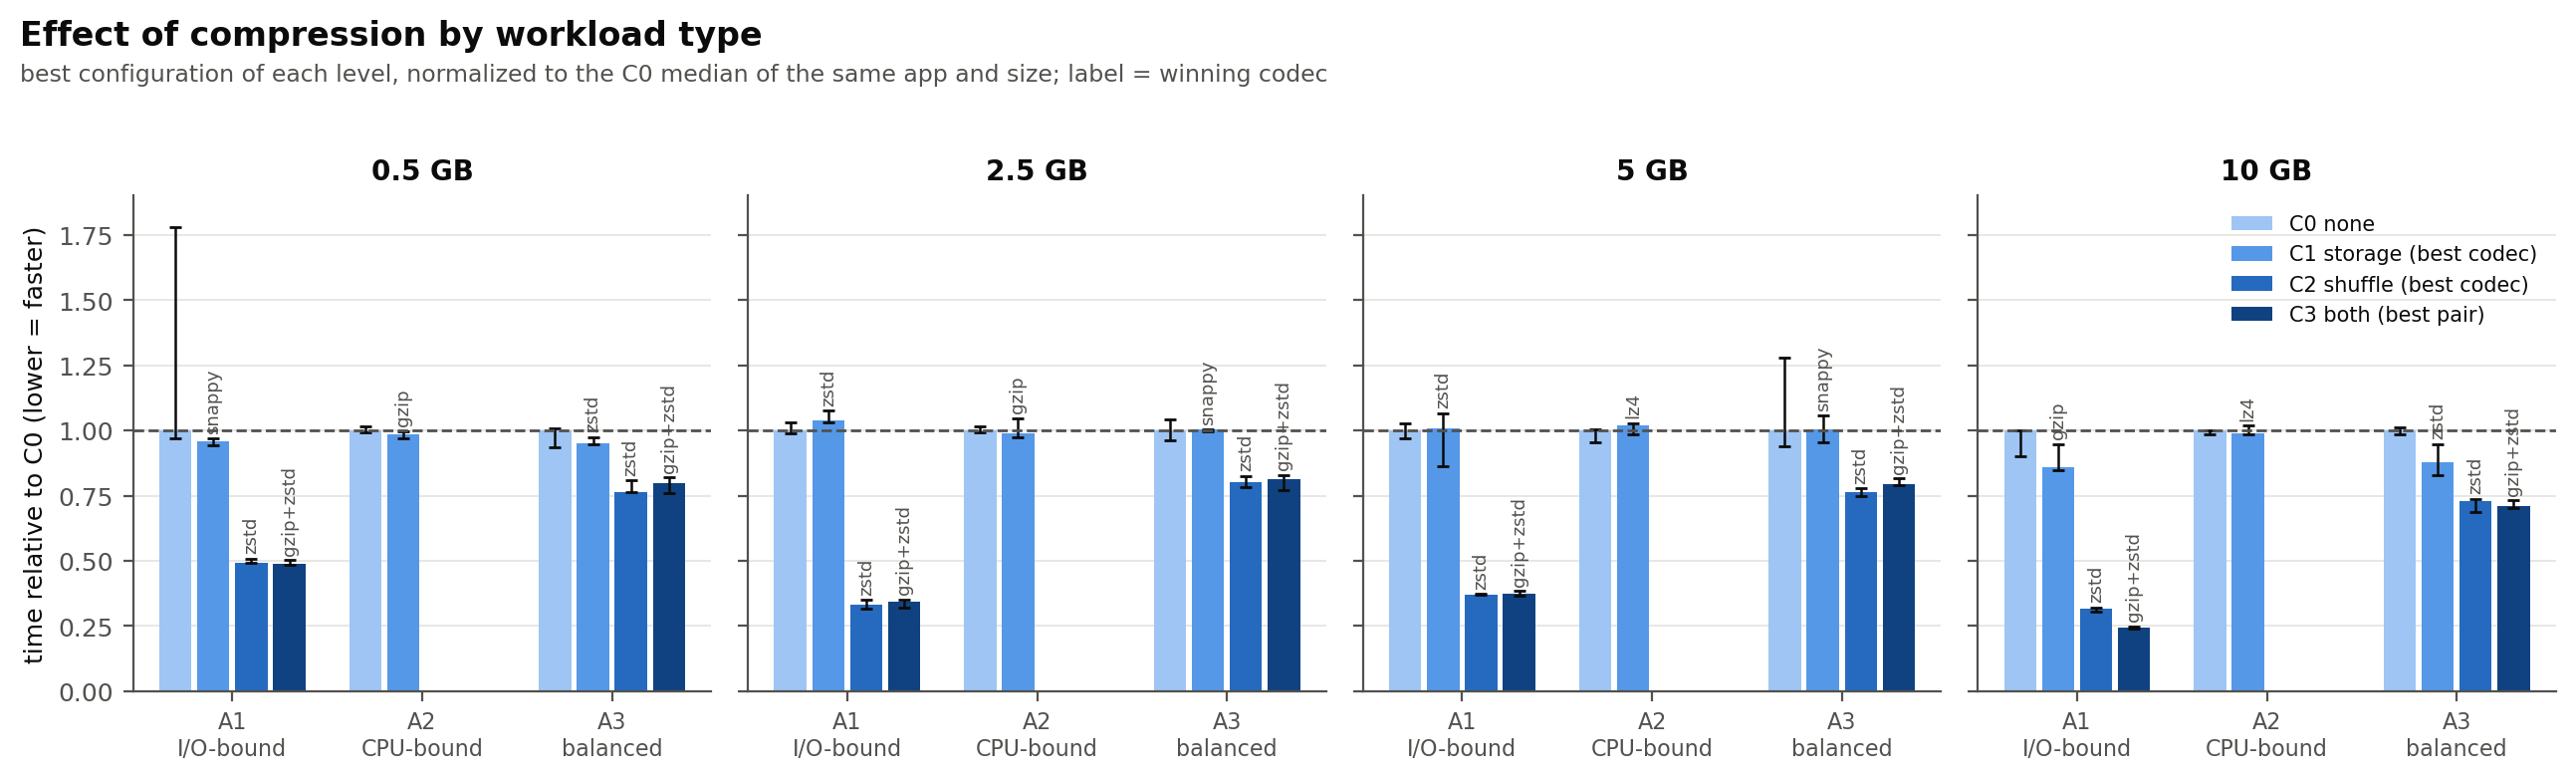
\includegraphics[width=\textwidth]{../results/plots/fig7_time_vs_workload.png}
    \end{column}

    \begin{column}{0.5\textwidth}
      \begin{block}{\footnotesize Q1: Best Ratio vs. CPU Trade-off?}
        \scriptsize
        \textbf{Zstandard (Zstd) at both levels.} Unmatched compression ratio among fast codecs, fractions of Gzip's CPU overhead. Gzip is dominated everywhere.
      \end{block}

      \begin{block}{\footnotesize Q2: Systematic Improvement in I/O-Bound Jobs?}
        \scriptsize
        \textbf{No.} Shuffle compression is systematic (up to 3.15$\times$); storage compression is not (only helps when input reading sits on the critical path).
      \end{block}

      \begin{block}{\footnotesize Q3: Effect on CPU-Bound Jobs (A2)?}
        \scriptsize
        \textbf{Zero benefit, minor penalty ($\pm 5\%$).} 4 of 16 cases had statistically significant 4--5\% slowdowns due to uncompensated decompression CPU.
      \end{block}
    \end{column}
  \end{columns}
\end{frame}

% -----------------------------------------------------------------------------
% Slide 12: Answers to Q4--Q7
% -----------------------------------------------------------------------------
\begin{frame}{Answers to Q4--Q7}
  \begin{columns}[T]
    \begin{column}{0.48\textwidth}
      \begin{block}{\footnotesize Q4: Evolution with Dataset Size?}
        \scriptsize
        Benefits grow with size as fixed costs amortize. Memory saturation at 10 GB triggers storage-level gains. Codec rankings remain invariant.
      \end{block}

      \begin{block}{\footnotesize Q5: Storage vs. Network Benefits?}
        \scriptsize
        \textbf{Network communication is far more beneficial.}
        \begin{itemize}
          \scriptsize
          \item Shuffle data is row-format (2.8--4.8$\times$ vs 1.4--1.9$\times$ for Parquet).
          \item Shuffle volume exceeds input ($4.3\times$ on A1).
          \item Wi-Fi link is the cluster's primary bottleneck.
        \end{itemize}
      \end{block}
    \end{column}

    \begin{column}{0.48\textwidth}
      \begin{block}{\footnotesize Q6: Can Combined Compression Degrade Performance?}
        \scriptsize
        \textbf{Yes, mildly.} When storage has nothing to save, it adds CPU overhead (Snappy+LZ4 was 16\% slower at 2.5 GB). Pays off only when both I/O paths are saturated.
      \end{block}

      \begin{alertblock}{\footnotesize Q7: When Should Compression Be Disabled?}
        \scriptsize
        \begin{enumerate}
          \scriptsize
          \item \textbf{CPU-bound workloads} (disable storage compression).
          \item \textbf{Small/medium datasets} on local NVMe storage.
          \item \textbf{Combined fast pairs} (\texttt{snappy+lz4}).
          \item \textbf{Gzip} under any CPU-constrained scenario.
        \end{enumerate}
      \end{alertblock}
    \end{column}
  \end{columns}
\end{frame}

% -----------------------------------------------------------------------------
% Slide 13: Threats to Validity, Outliers & Limitations
% -----------------------------------------------------------------------------
\begin{frame}{Threats to Validity, Outliers \& Limitations}
  \begin{columns}[T]
    \begin{column}{0.5\textwidth}
      \centering
      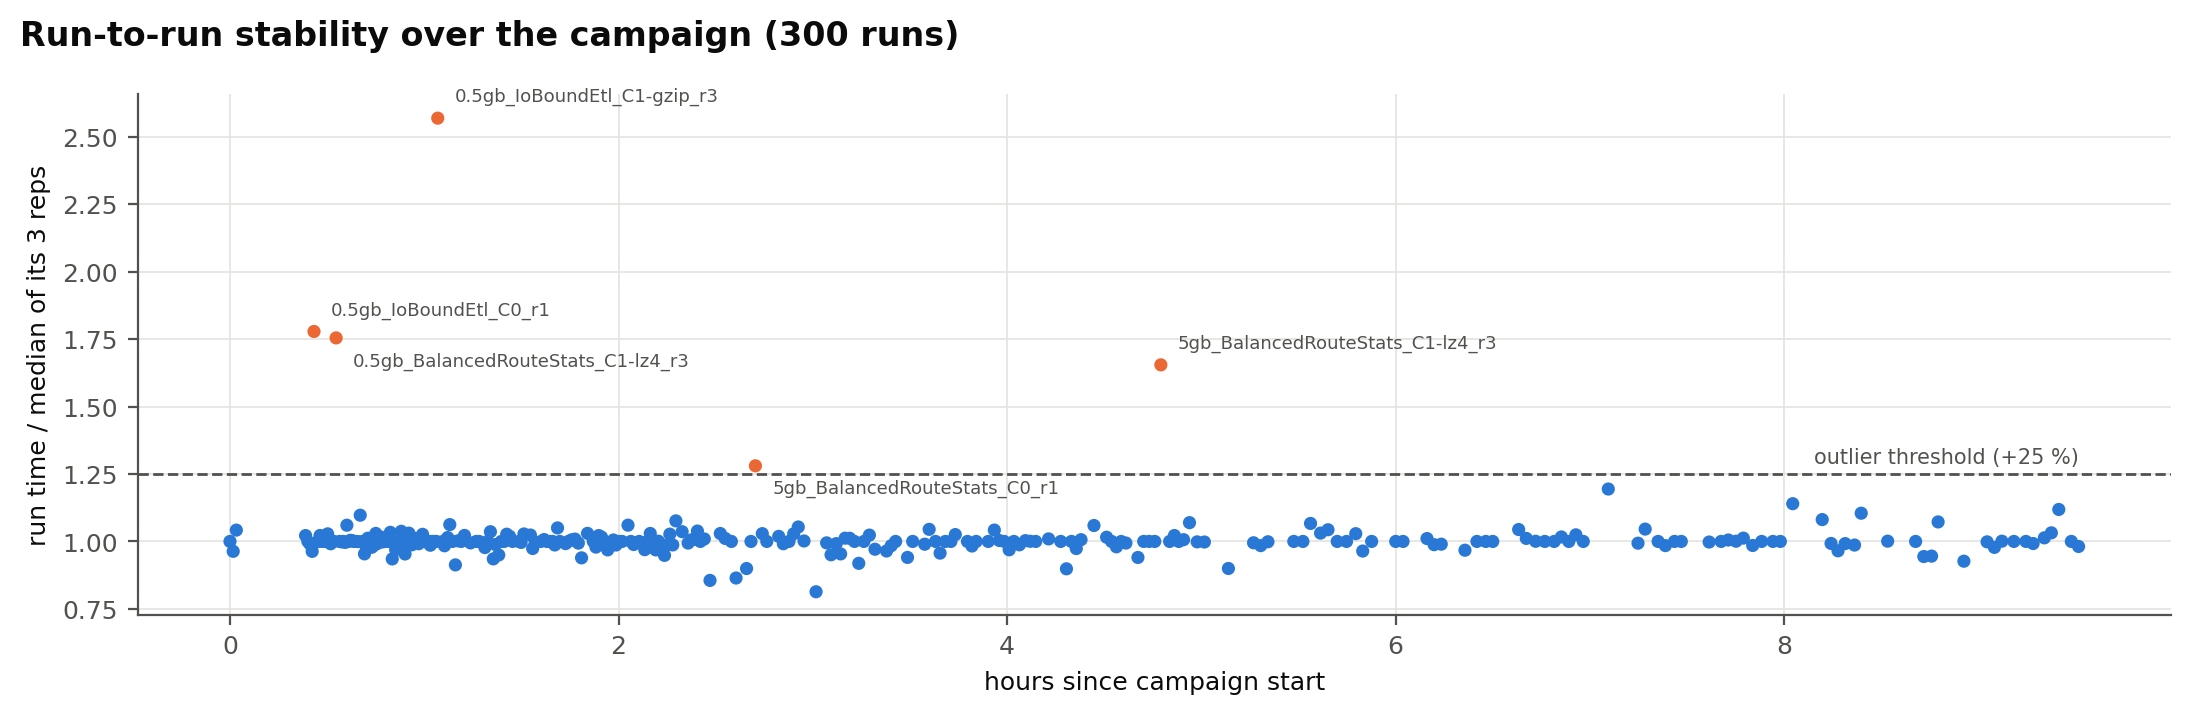
\includegraphics[width=\textwidth]{../results/plots/fig9_stability.png}
    \end{column}

    \begin{column}{0.48\textwidth}
      \textbf{Critical Analysis \& Limitations:}
      \begin{itemize}
        \footnotesize
        \item \textbf{Wi-Fi Interconnect vs Datacenter:}
          \begin{itemize}
            \scriptsize
            \item Home Wi-Fi link (300--600 Mbit/s) amplifies shuffle compression gains.
            \item On 10--25 GbE enterprise networks, shuffle speed-ups would be narrower.
          \end{itemize}
        \item \textbf{Hardware Asymmetry:}
          \begin{itemize}
            \scriptsize
            \item 16 PC cores vs 4 Mac VM cores; 80\% of tasks execute on PC.
          \end{itemize}
        \item \textbf{Outlier Analysis (5 of 300 runs):}
          \begin{itemize}
            \scriptsize
            \item 5 runs were $>25\%$ slower due to Mac executor stragglers (two 60 s HDFS connect timeouts, three VM thread stalls).
            \item \textbf{Methodological rigor:} Outliers were kept; reporting \textbf{medians with min..max bars} preserved robustness.
          \end{itemize}
      \end{itemize}
    \end{column}
  \end{columns}
\end{frame}

% -----------------------------------------------------------------------------
% Slide 14: Practical Engineering Guidelines for Spark
% -----------------------------------------------------------------------------
\begin{frame}{Practical Engineering Guidelines for Spark}
  \begin{columns}[T]
    \begin{column}{0.48\textwidth}
      \begin{exampleblock}{1. Always Enable Shuffle Compression}
        \begin{itemize}
          \scriptsize
          \item Default \texttt{lz4} is excellent for high-speed networks.
          \item Switch to \textbf{Zstandard (\texttt{zstd}, level 1)} whenever network bandwidth is constrained or clusters are oversubscribed.
        \end{itemize}
      \end{exampleblock}

      \begin{exampleblock}{2. Default Parquet Storage to Zstd}
        \begin{itemize}
          \scriptsize
          \item Set \texttt{spark.sql.parquet.compression.codec=zstd} (level 3).
          \item Replaces both Snappy and Gzip as the modern storage standard.
        \end{itemize}
      \end{exampleblock}
    \end{column}

    \begin{column}{0.48\textwidth}
      \begin{alertblock}{3. Never Use Gzip in Big Data Pipelines}
        \begin{itemize}
          \scriptsize
          \item 10$\times$ slower than Zstd at compression.
          \item Adds up to +62\% CPU overhead with no compression ratio benefit on columnar Parquet data.
        \end{itemize}
      \end{alertblock}

      \begin{block}{4. Profile Bottlenecks First}
        \begin{itemize}
          \scriptsize
          \item Compressing storage data at rest does not speed up jobs if input I/O is not on the critical path.
          \item For CPU-bound pipelines, leave storage compression disabled or use lightweight LZ4.
        \end{itemize}
      \end{block}
    \end{column}
  \end{columns}
\end{frame}

% -----------------------------------------------------------------------------
% Slide 15: Conclusion & Q&A
% -----------------------------------------------------------------------------
\begin{frame}[c]{Conclusion \& Q\&A}
  \centering
  \Large
  \textbf{Thank You for Your Attention!}\\[0.4cm]

  \normalsize
  \textbf{Experimental Summary:}
  \begin{itemize}
    \centering
    \small
    \item 300 runs on a 20-core heterogeneous cluster with 100\% reproducibility.
    \item Demonstrated that shuffle compression is the dominant performance lever.
    \item Zstandard established as the superior algorithm across both storage and shuffle tiers.
  \end{itemize}

  \vspace{0.4cm}
  \large
  \textbf{Questions \& Discussion}
\end{frame}

\end{document}
